\section{Magnetic resonance imaging}\label{sec:mri}
While the previous imaging modalities were based on X-rays, Magnetic Resonance
Imaging (MRI) is based on magnetic fields. It is sometimes also referred to as
Nuclear Magnetic Resonance (NMR) in professional circles. However, the general
public has a certain aversion to the world ``nuclear'', so MRI is most used.
Instead of measuring the electromagnetic attenuation properties of various
tissue types as in CT scanners, we measure certain magnetic properties of the
tissue. These magnetic properties mainly depend on the molecular composition of
the material, for example on the amount of H$^+$ ions present (the proton
density). These electromagnetic waves are non-ionizing, meaning they cannot
cause cancer due to prolonged exposure. The goal is the same: imaging slices of
a patient's body. While technically an MRI scanner can generate slices in any
orientation without even moving the patient, CT-like cross sectional slices
are still used predominantly. Figure \ref{fig:mriscanner} shows a picture of an MRI
scanner.

\begin{figure}[ht]
\begin{center}
  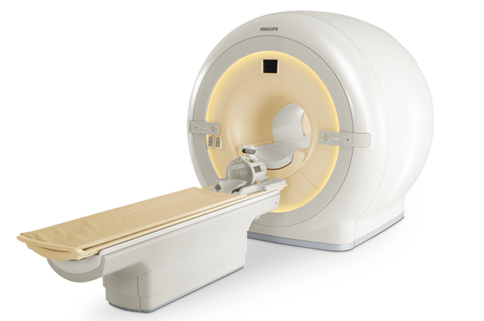
\includegraphics[width=\linewidth]{img/mriscanner.jpg}
  \caption{A Phlips MRI scanner. The patient takes place on the bed and is
  moved inside the toroid, but is not moved again during the procedure.}
  \label{fig:mriscanner}
\end{center}
\end{figure}

\subsection{History}\label{ssec:mrihist}
During the late 1960's, researcher in Aberdeen worked on the predecessor of the
modern MRI scanner \cite{mrihistory}. Their goal was to distinguish between
malignant tumors and normal tissue without using ionizing radiation. Instead of
measuring the magnetic properties of the nuclei, they initially focused on
electrons. This proved to be a dead end, and by early 1970 the group moved on to
NMR as we know it today. They realized that tumors have a longer $T_1$ time
(see below), and concentrated on that instead.

Meanwhile in the USA, chemist Paul Lauterbur proposed a way to create images
from NMR studies by using multiple field gradients to encode the position of
each measurement \cite{lauterbur1973}. Another important contribution came from
Peter Mansfield (now Sir), an English physicist. In 1974, he showed how to
select spins from a specific slice and patented a method to selectively excite
and define a slice across a sample. Lauterbur and Mansfield shared the 2003
Nobel Prize in Physiology or Medicine for their work on NMR.

From 1978 on, multiple research groups started presenting images generated by
prototype MRI scanners. However, only in the early 1980's was the technology 
ready for clinical and diagnostic use. By 1983, major multinational corporations
started producing commercial MRI machines.

\subsection{Technical background}
Unfortunately, the fundamental concepts that make MRI scanners work go beyond
classic physics, and instead requires special relativity, quantum mechanics and
quantum electrodynamics. Clearly, this is way beyond the scope of this text. We
will present a simplified version of the core principles based on
\cite{suetens} instead.

MRI scanners influence and measure the magnetic properties of atom nuclei in the
patient's tissue. During typical studies H$^+$ ions (i.e., protons) are used
because of their abundance in the human body, although alternatives exist
(e.g. ${}^{13}_6$C or ${}^{17}_8$O).

When the scanner is operational, a large magnetic field $\vec{B_0} = (0,0,B_0)$
(in the order of a couple Telsa) is induced along the patient's length using a
big electromagnetic coil. By supercooling the coil, the resistance drops and
power consumption can be reduced significantly.

The magnetic field $\vec{B_0}$ influences the magnetic moments $\vec{\mu_i}$ of
the nuclei, causing them to precess around the z-axis with precession frequency
$\omega_0 = f(B_0)$. Associated with the external magnetic field and the
individuel magnetic moments is the potential energy $E$. Quantum mechanics
states that for protons, this energy can only have two values, the so-called
spin up ($E_\uparrow$, lowest) and spin down ($E_\downarrow$, highest) state. In
these states, the $\vec{\mu_i}$ point respectively upwards ($u_z > 0$) and
downwards ($u_z < 0$), although transverse components are still present. Most
protons will be in the lowest energy state, but they can be flipped by absorbing
a photon with the appropriate amount of energy $\Delta E = E_\downarrow -
E_\uparrow$. This holds when the photon has a specific Larmor frequency
$\omega_{RF}$, which happens to be equal to $\omega_0$. In a 1T field, the
Larmor frequency for hydrogen is 42.6 MHz, a radio-frequency (RF) wave.

Of course, we are more interested in macroscopic voxels (3D pixels) than in the
individual nuclei. Fortunately, the net magnetization vector $\vec{M_0}$ of each
voxel is simply the sum of all individual magnetic moments $\mu_i$. The
magnitude of this vector roughly represents the proton density in the voxel. In
dynamic equilibrium, $\vec{M_0}$ points in the same direction as $\vec{B_0}$
because there are more nuclei in the spin up state and the individual transverse
components cancel each other out. To summarize: the large magnetic field made
sure the net magnetization vectors of all voxels are aligned. 

Unfortunately, due to technical reasons we can only measure the transverse
component of $\vec{M}$. As a solution, we will disturb the dynamic equilibrium
with a resonating RF pulse, causing more protons to flip to the spin down state.
This RF wave has a magnetic component $\vec{B_1} = (B_1, 0, 0)$. Following the
same logic as above, $\vec{B_1}$ causes $\vec{M}$ to precess around it. With the
appropriate timing, $\vec{M}$ can be flipped over an angle $\alpha$ of either 90
or 180 degrees.

After the pulse, the system returns to dynamic equilibrium during a process
called relaxation. We can distinguish between two effects. First, spin-spin
relaxation is responsible for the disappearance of the transverse component of
the net magnetization vector due to loss of phase coherence (increase in
entropy while energy stays constant). This process can easily be approximated
by a first order model with a time constant $T_2$, called the spin-spin
relaxation time.

\begin{equation}
M_{tr}(t) = M_0 \sin(\alpha) e^{-t/T_2}
\end{equation}

Different tissue types have different inherent $T_2$ times, which we will
exploit later.

\begin{figure}[ht]
\begin{center}
  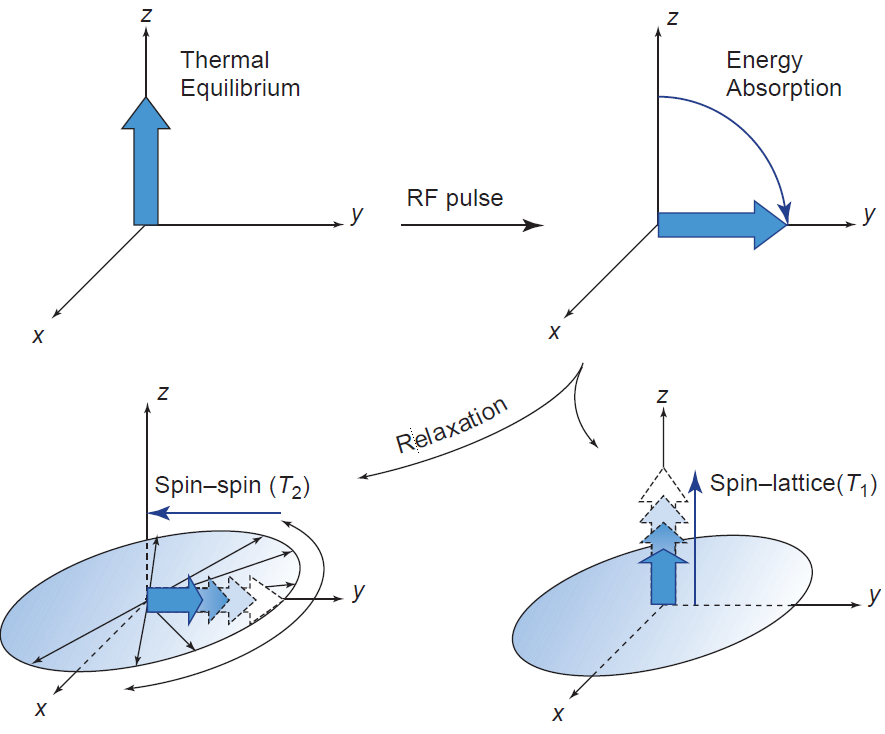
\includegraphics[width=\linewidth]{img/relaxation.png}
  \caption{Schematic overview of relaxation after a 90 degree pulse. \cite{suetens}}
  \label{fig:relaxation}
\end{center}
\end{figure}

Second, spin-lattice relaxation is responsible for regenerating the
longitudinal component of $\vec{M}$. Similarly, this process can be linked to a
$T_1$ relaxation time. $T_1$ is also a tissue property, and is always larger
than $T_2$.

\begin{equation}
M_l(t) = M_0 \cos(\alpha) e^{-t/T_1} + M_0 (1 - e^{-t/T_1})
\end{equation}

Using a quadrature detector in the xy-plane, we get the following reading
after one 90 degree pulse:
\begin{equation}
s(t) = M_{tr}(t) = M_0 e^{-t/T_2}
\end{equation}

To also measure $T_1$, we have to repeat the 90 degree pulse after repetition
time TR:
\begin{equation}
s(t) = M_0 (1 - e^{-TR/T_1}) e^{-t/T_2}
\end{equation}

Notice how the 90 degree pulse conveniently eliminates the sine and cosine
factors.

Clearly the result is not just the proton density $M_0$, but involves other
factors as well. This is not necessarily a problem as the $T_1$ and $T_2$
factors can increase the discriminative power of the scanner. If a short $TR$ is
chosen, the image is said to be $T_1$ weighted because long $TR$ times cause the
$T_1$ factor to diminish. If on the other hand a long $TE$ (echo time = moment
of measurement) is chosen, the image is said to be $T_2$ weighted. Indeed, a
short $TE$ time decreases the $T_2$ factor. By combining a long $TR$ with a
short $TE$, we have a relatively pure proton density image. Remember that $TR$
and $TE$ can be chosen by the operator, while $T_1$ and $T_2$ are tissue
dependent.

The attentive reader will have noticed that there is no spatial information
encoded in this signal yet. Using this approach we could only measure the
combined effects of all relaxations, which is useless. To solve this, we
superimpose additional gradients $\vec{G}_{x/y/z}$ (in the order of
milliTesla/meter) onto $\vec{B_0}$. This in turn affects the Larmor frequency.
The exact details are far from trivial and will be omitted, but involve the
3D k-space. After the signal has been sampled everywhere in the region of
interest in the k-space, a simple inverse Fourier transformation yields the
image we are looking for.

Using two 90 degree pulses is just one of the many possible pulse sequences used
in modern MRI scanners. Other examples include the spin-echo (SE) sequence and
the gradient echo (GE) sequence. Each sequence has advantages and disadvantages
with respect to discrimination of certain tissue types. The radiologist is
responsible for making the proper choice.

%fMRI (oxygen T2)
%flexible

\subsection{Recent advancements}
A lot of spin-off technologies based on MRI are in use. For example, Magnetic
Resonance Angiography (MRA) generates pictures of arteries to detect pathologies
such as stenosis (narrowing) or aneurysms (dilations). To make this work the
patient can be injected with a paramagnetic material. Alternatively, the scanner
can detect anomalies in the measurements due to movement of the blood, and
amplify those.

\hyphenation{me-ta-bo-lites}

Similarly, Magnetic Resonance Spectroscopy (MRS) measures the levels of various
metabolites in human tissue, while functional MRI (fMRI) visualizes brain
activity based on local oxygen levels. The underlying principle is that
oxygen-rich blood contains oxyhemoglobin, which is diamagnetic, while
oxygen-poor blood containing deoxyhemoglobin is paramagnetic. Likewise,
diffusion and perfusion can be measured.

\subsection{Future expectations}\label{ssec:mrifuture}
MRI scanners today are still far less ubiquitous than CT scanners, and only make
up a few percent of the worldwide radiographic examinations \cite{oecdhealth}.
However, because of the various advantages over other modalities - mostly the
fact that they use non-ionizing radiation - usage is expected to rise steadily
in the future. MRI will never completely replace CT because it cannot properly
image hydrogen-poor structures such as bone and air.

On top of that, future research will most likely improve the functional aspect
(e.g. measuring blood flow) of MRI. This can be done by experimenting with
nuclei other than hydrogen, by using new contrast agents and using novel pulse
sequences. In addition - similar to CT scanners - research will try to increase
the contrast and lower the acquisition times even further.